%\documentclass[landscape,a0b,final,a4resizeable]{a0poster}
\documentclass[landscape,a0b,final]{a0poster}
%\documentclass[portrait,a0b,final,a4resizeable]{a0poster}
%\documentclass[portrait,a0b,final]{a0poster}
%%% Option "a4resizeable" makes it possible to resize the
%   poster by the command: psresize -pa4 poster.ps poster-a4.ps
%   For final printing, please remove option "a4resizeable" !!

\usepackage{epsfig}
\usepackage{multicol}
\usepackage{pstricks,pst-grad}
\usepackage{graphicx,psfrag}
\usepackage{graphics}
\usepackage{amsmath}
\usepackage{amsthm}
\usepackage{amsfonts}

\newtheorem{example}{Example}
\newtheorem{assumption}{Assumption}
\newtheorem{definition}{Definition}
\newtheorem{theorem}{Theorem}
\newtheorem{lemma}{Lemma}


%%%%%%%%%%%%%%%%%%%%%%%%%%%5

\usepackage{eso-pic}
\usepackage{graphicx}
\usepackage{color}
\usepackage{type1cm}


%%%%%%%%%%%%%%%%%%%%%%%%%%%%%%%%%%%%%%%%%%%%%%%%%%%%
%%%               WaterMark                       %%%
%%%%%%%%%%%%%%%%%%%%%%%%%%%%%%%%%%%%%%%%%%%%%%%%%%%%
%\makeatletter
%  \AddToShipoutPicture{%
%    \setlength{\@tempdimb}{.5\paperwidth}%
%    \setlength{\@tempdimc}{.5\paperheight}%
%    \setlength{\unitlength}{1pt}%
%    \put(\strip@pt\@tempdimb,\strip@pt\@tempdimc){%
%      \makebox(0,0){\rotatebox{45}{\textcolor[gray]{0.15}{
\includegraphics[width=120cm,angle=0]{SU_Seal_Card_pos.eps}}}}
%    }
%}
%\makeatother



%%%%%%%%%%%%%%%%%%%%%%%%%%%%%%%%%%%%%%%%%%%
% Definition of some variables and colors
%\renewcommand{\rho}{\varrho}
%\renewcommand{\phi}{\varphi}
\setlength{\columnsep}{3cm}
\setlength{\columnseprule}{2mm}
\setlength{\parindent}{0.0cm}



%%%%%%%%%%%%%%%%%%%%%%%%%%%%%%%%%%%%%%%%%%%%%%%%%%%%
%%%               Background                     %%%
%%%%%%%%%%%%%%%%%%%%%%%%%%%%%%%%%%%%%%%%%%%%%%%%%%%%

\newcommand{\background}[3]{
  \newrgbcolor{cgradbegin}{#1}
  \newrgbcolor{cgradend}{#2}
  \psframe[fillstyle=gradient,gradend=cgradend,
  gradbegin=cgradbegin,gradmidpoint=#3](0.,0.)(1.\textwidth,-1.\textheight)
}



%%%%%%%%%%%%%%%%%%%%%%%%%%%%%%%%%%%%%%%%%%%%%%%%%%%%
%%%                Poster                        %%%
%%%%%%%%%%%%%%%%%%%%%%%%%%%%%%%%%%%%%%%%%%%%%%%%%%%%

\newenvironment{poster}{
  \begin{center}
  \begin{minipage}[c]{0.98\textwidth}
}{
  \end{minipage} 
  \end{center}
}



%%%%%%%%%%%%%%%%%%%%%%%%%%%%%%%%%%%%%%%%%%%%%%%%%%%%
%%%                pcolumn                       %%%
%%%%%%%%%%%%%%%%%%%%%%%%%%%%%%%%%%%%%%%%%%%%%%%%%%%%

\newenvironment{pcolumn}[1]{
  \begin{minipage}{#1\textwidth}
  \begin{center}
}{
  \end{center}
  \end{minipage}
}



%%%%%%%%%%%%%%%%%%%%%%%%%%%%%%%%%%%%%%%%%%%%%%%%%%%%
%%%                pbox                          %%%
%%%%%%%%%%%%%%%%%%%%%%%%%%%%%%%%%%%%%%%%%%%%%%%%%%%%

%\newrgbcolor{lcolor}{0. 0. 0.80}
\newrgbcolor{lcolor}{1 1 1}
\newrgbcolor{gcolor1}{1. 1. 1.}
\newrgbcolor{gcolor2}{.80 .80 1.}

\newcommand{\pbox}[4]{
\psshadowbox[#3]{
\begin{minipage}[t][#2][t]{#1}
#4
\end{minipage}
}}



%%%%%%%%%%%%%%%%%%%%%%%%%%%%%%%%%%%%%%%%%%%%%%%%%%%%
%%%                myfig                         %%%
%%%%%%%%%%%%%%%%%%%%%%%%%%%%%%%%%%%%%%%%%%%%%%%%%%%%
% \myfig - replacement for \figure
% necessary, since in multicol-environment 
% \figure won't work

\newcommand{\myfig}[3][0]{
\begin{center}
  \vspace{1.5cm}
  \includegraphics[width=#3\hsize,angle=#1]{#2}
  \nobreak\medskip
\end{center}}

\newcommand{\myfigp}[3][0]{
\begin{center}
  \vspace{1.5cm}
  \includegraphics[width=#3\hsize]{#1}
  \includegraphics[width=#3\hsize]{#2}
  \nobreak\medskip
\end{center}}



%%%%%%%%%%%%%%%%%%%%%%%%%%%%%%%%%%%%%%%%%%%%%%%%%%%%
%%%                mycaption                     %%%
%%%%%%%%%%%%%%%%%%%%%%%%%%%%%%%%%%%%%%%%%%%%%%%%%%%%
% \mycaption - replacement for \caption
% necessary, since in multicol-environment \figure and
% therefore \caption won't work

%\newcounter{figure}
\setcounter{figure}{1}
\newcommand{\mycaption}[1]{
  \vspace{0.5cm}
  \begin{quote}
    {{\sc Figure} \arabic{figure}: #1}
  \end{quote}
  \vspace{1cm}
  \stepcounter{figure}
}



%%%%%%%%%%%%%%%%%%%%%%%%%%%%%%%%%%%%%%%%%%%%%%%%%%%%%%%%%%%%%%%%%%%%%%
%%% Begin of Document
%%%%%%%%%%%%%%%%%%%%%%%%%%%%%%%%%%%%%%%%%%%%%%%%%%%%%%%%%%%%%%%%%%%%%%

\begin{document}





\newrgbcolor{lightblue}{0. 0. 0.80}
\newrgbcolor{white}{1. 1. 1.}
\newrgbcolor{whiteblue}{1 1 1}
\newrgbcolor{red}{0.6431 0 0.1137}
\newrgbcolor{whitered}{0.6431 0 0.1137}




\begin{poster}

\background{0.6431 0 0.1137}{1. 1. 1.}{0.5}
\vspace*{2.5cm}
%%%%%%%%%%%%%%%%%%%%%
%%% Header
%%%%%%%%%%%%%%%%%%%%%
\begin{center}
\begin{pcolumn}{0.992}

\pbox{0.95\textwidth}{}{linewidth=4mm,framearc=0.3,linecolor=red,fillstyle=gradient,gradangle=0,gradbegin=white,gradend=white,gradmidpoint=1.0,framesep=1em}{

%%% DARPA-DSO logo
\begin{minipage}[c][4.5cm][c]{0.13\textwidth}
  \begin{center}
    
\includegraphics[width=13cm,angle=0]{Darpadsologo}
  \end{center}
\end{minipage}
%%% AA logo
\begin{minipage}[c][4.5cm][c]{0.14\textwidth}
  \begin{center}
    %
\includegraphics[width=8cm,angle=0]{SU_Seal_Card_pos}
    \vspace{5mm}
    
\includegraphics[width=12cm,angle=0]{aalogo}
  \end{center}
\end{minipage}
%%% Title
\begin{minipage}[c][9cm][c]{0.46\textwidth}
  \begin{center}
    {\sc \Huge Cutoff Phenomena in Chaotic Dynamics}\\[10mm]
    {\Large Tzu-Chen Liang\\[7.5mm]
     Department of Aeronautics and Astronautics, Stanford University }
  \end{center}
\end{minipage}
%%% Stanford logo
\begin{minipage}[c][4.5cm][c]{0.10\textwidth}
  \begin{center}
    \hspace{2cm}
    
\includegraphics[width=8cm,angle=0]{SU_Seal_Card_pos}
  \end{center}
\end{minipage}
%%% DynaRUM logo
\begin{minipage}[c][9cm][c]{0.17\textwidth}
  \begin{center}
    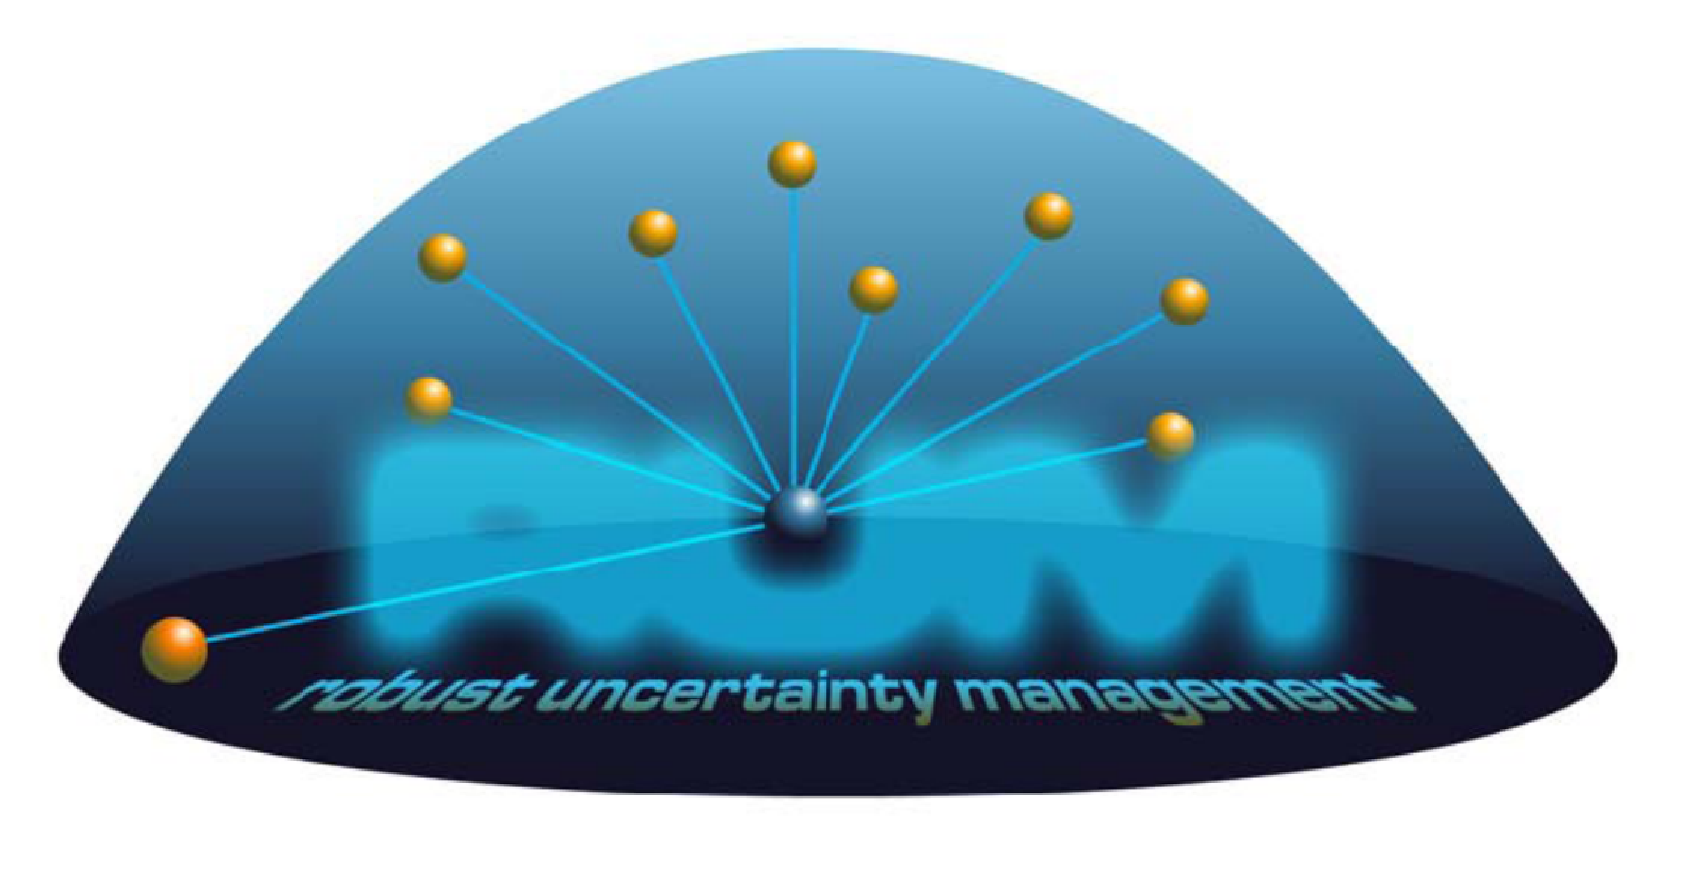
\includegraphics[width=15cm,angle=0]{Dynarumlogo}
  \end{center}
\end{minipage}
} 



%\pbox{0.95\textwidth}{}{linewidth=4mm,framearc=0.3,linecolor=red,fillstyle=gradient,gradangle=0,gradbegin=white,gradend=white,gradmidpoint=1.0,framesep=1em}{








\end{pcolumn}
\end{center}


\vspace*{2cm}



%%%%%%%%%%%%%%%%%%%%%
%%% Content
%%%%%%%%%%%%%%%%%%%%%
%%%%%%%%%%%%%%%%%%%%%%%%%%%%%%%%
%Here is the 1st column
%%%%%%%%%%%%%%%%%%%%%%%%%%%%%%%%

\begin{center}
\begin{pcolumn}{0.32}
\pbox{0.9\textwidth}{65cm}{linewidth=4mm,framearc=0.1,linecolor=red,fillstyle=gradient,gradangle=0,gradbegin=white,gradend=white,gradmidpoint=1.0,framesep=1em}{

%%% Introduction
\begin{center}\pbox{0.8\textwidth}{}{linewidth=2mm,framearc=0.1,linecolor=red,fillstyle=gradient,gradangle=0,gradbegin=white,gradend=whitered,gradmidpoint=1.0,framesep=1em}{\begin{center}\bfseries{\large{Introduction}}\end{center}}\end{center}
\vspace{1.25cm}
%%%%%%%%%%%%%%%%%%%%%%%%%%%%%%%%%%%%%%%%%%%%%%%%%%%%%%%%%%%%%%%%%%%%%%%%%%%%%%%%%%%%%%%%%%%%%%%%
%Introduction begins here
\begin{itemize}
 \item Prove the scalar measure of certainty/uncertainty can have a phase change(cutoff) under chaotic mapping. 
 \item Show the dual relation between chaotic mixing and chaotic randomizing.
 \item Numerical evidence of cutoff is provided for 2-D standard map and a linked twist map with small diffusion. 
\end{itemize}

\begin{tabular}{c|l}
  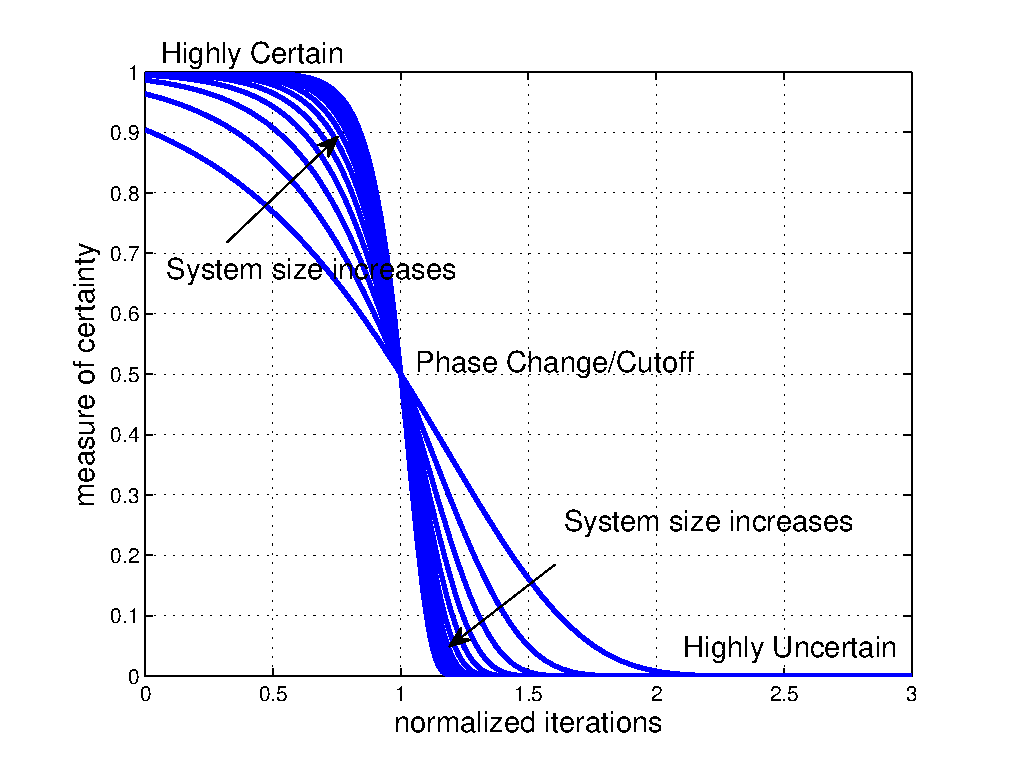
\includegraphics[width=0.55\hsize]{democutoffn}&
  \begin{minipage}[b]{0.43\hsize}
  \paragraph{The phase change of scalar measure of certainty}
  The scalar measure of certainty changes sharply from $1$ to $0$, which indicates the state of the system evolves from highly certain to highly uncertain. This tendency is reinforced when system size becomes larger, and thus presents a cutoff or a sharp phase change under the normalized plot.   
  \end{minipage}
\end{tabular}

%Introduction ends here
%%%%%%%%%%%%%%%%%%%%%%%%%%%%%%%%%%%%%%%%%%%%%%%%%%%%%%%%%%%%%%%%%%%%%%%%%%%%%%%%%%%%%%%%%%%%%%%%%




%%% Cutoff 
\vspace{0.7cm}\begin{center}\pbox{0.8\textwidth}{}{linewidth=2mm,framearc=0.1,linecolor=red,fillstyle=gradient,gradangle=0,gradbegin=white,gradend=whitered,gradmidpoint=1.0,framesep=1em}{\begin{center}\bfseries{\large{Cutoff Phenomenon}}\end{center}}\end{center}\vspace{1cm}
%%%%%%%%%%%%%%%%%%%%%%%%%%%%%%%%%%%%%%%%%%%%%%%%%%%%%%%%%%%%%%%%%%%%%%%%%%%%%%%%%%%%%%%%%%%%%%%%
%section begins here

We state the definition of a cutoff given by Diaconis in
\cite{Diaconis2005}. Assume that, to any finite set $\Omega$ and any
pair of probability measures $\omega$, $\bar{\omega}$ on $\Omega$ is associated
a real number $D(\omega,\bar{\omega})$ such that $D(\omega,\bar{\omega})\in [0,1]$,
%\begin{eqnarray}
$\max_{\{\Omega,\omega,\bar{\omega}\}} D(\omega,\bar{\omega}) = 1$, 
%\end{eqnarray}
and $D(\omega,\bar{\omega})=0$ if and only if $\bar{\omega}=\omega$. Consider a sequence of
(finite) probability spaces $(\Omega_n,\bar{\omega}_n)$, $n=1,2,...$, each
equipped with a sequence of probability measure $\omega^k_n$,
$l=0,1,...$, such that
%\begin{eqnarray}
$\lim_{k \rightarrow \infty} D(\omega_n,\bar{\omega}_n)=0$.
%\end{eqnarray}
The definition of a cutoff is,

\begin{definition}
\label{cutoffdefinition}
(Diaconis) A family $(\Omega_n,\bar{\omega}_n, (\omega^k_n)_{k=0,1,...})_{n=1,2,...}$
presents a D-cutoff if there exists a sequence $(t_n)$ of positive
reals such that, for any $\epsilon \in(0,1)$,
\begin{enumerate}
  \item $\lim_{n \rightarrow \infty}D(\omega^{k_n}_n,\bar{\omega}_n) = 0 \mbox{ if }
  k_n>(1+\epsilon)t_n$
  \item $\lim_{n \rightarrow \infty}D(\omega^{k_n}_n,\bar{\omega}_n) = 1 \mbox{ if }
  k_n<(1-\epsilon)t_n $
\end{enumerate}
\end{definition}

We relax the definition and set $\Omega_n$ to be infinite. We say that a family $(\Omega_n,\bar{\omega}_n, (\omega^k_n)_{k=0,1,...})_{n=1,2,...}$ presents a D-cutoff in the relaxed sense if it satisfies definition \ref{cutoffdefinition} but $\Omega_n$ is infinite. 


The distance measure we are interested in is the following: 
\vspace{-0.8cm}

\paragraph{Total Variation Distance}
  \begin{eqnarray*}
   \|\omega^k - \bar{\omega}\|_{TV} = \frac{1}{2}\sum_{i=1}^n |\omega_i^k-\bar{\omega}_i |= \frac{1}{2}\sum_{i=1}^n |f_i^k-1|\bar{\omega}_i
  \end{eqnarray*}
  where $f^k_i = \omega_i^k/\bar{\omega}_i$. $f$ is the density of $\omega$ with respect to $\bar{\omega}$.

\begin{example} \textbf{Random walk on an $n$-dimensional hypercube          }

 \vspace{0.3cm}
  \begin{tabular}{c|l}
     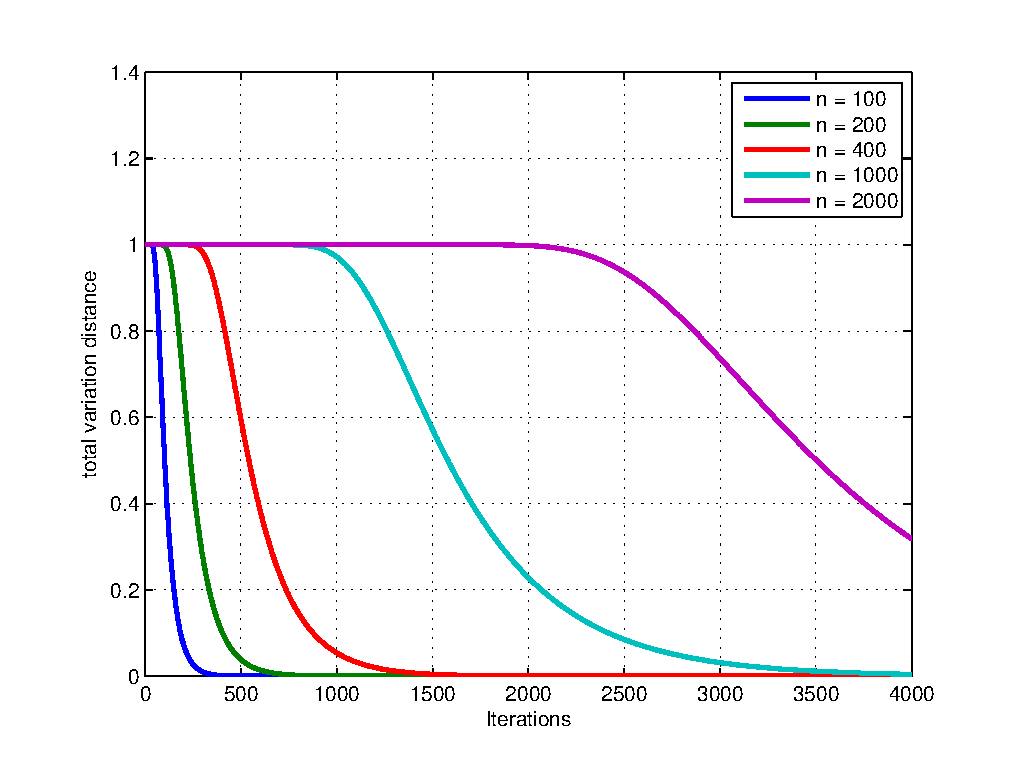
\includegraphics[width=0.4\hsize]{rdwalk.eps} &
     \begin{minipage}[b]{0.58\hsize}
          A particle starts at $\mathbf{0}$ and moves to one of its nearest neighbors (or stays fixed) with equal probability at each step.
    
          [Diaconis 1990] proves the following statement: 
          Let $k = \frac{1}{4}n\log{n}+cn$. Then for fixed $c \in \{-\infty,\infty\}$, as $n \rightarrow \infty$,
        \begin{eqnarray}
        \label{rdwalkshape}
            |\omega^k_n - \bar{\omega} |_{TV} \sim \text{Erf}\left(\frac{e^{-2c}}{\sqrt{8}}\right)
        \end{eqnarray}
     \end{minipage}
   \end{tabular}
\end{example}



%section ends here
%%%%%%%%%%%%%%%%%%%%%%%%%%%%%%%%%%%%%%%%%%%%%%%%%%%%%%%%%%%%%%%%%%%%%%%%%%%%%%%%%%%%%%%%%%%%%%%%%





}
\end{pcolumn}
\begin{pcolumn}{0.32}
%%%%%%%%%%%%%%%%%%%%%%%%%%%%%%%%
%Here is the 2nd column
%%%%%%%%%%%%%%%%%%%%%%%%%%%%%%%%
\pbox{0.9\textwidth}{65cm}{linewidth=4mm,framearc=0.1,linecolor=red,fillstyle=gradient,gradangle=0,gradbegin=white,gradend=white,gradmidpoint=1.0,framesep=1em}{



\begin{center}\pbox{0.8\textwidth}{}{linewidth=2mm,framearc=0.1,linecolor=red,fillstyle=gradient,gradangle=0,gradbegin=white,gradend=whitered,gradmidpoint=1.0,framesep=1em}{\begin{center}\bfseries{\large{Tent Map and Logistic Map "Cutoffs"}}\end{center}}\end{center}\vspace{1cm}

%%%%%%%%%%%%%%%%%%%%%%%%%%%%%%%%%%%%%%%%%%%%%%%%%%%%%%%%%%%%%%%%%%%%%%%%%%%%%%%%%%%%%%%%%%%%%%%%
%Section begins here

\begin{tabular}{c|l}
  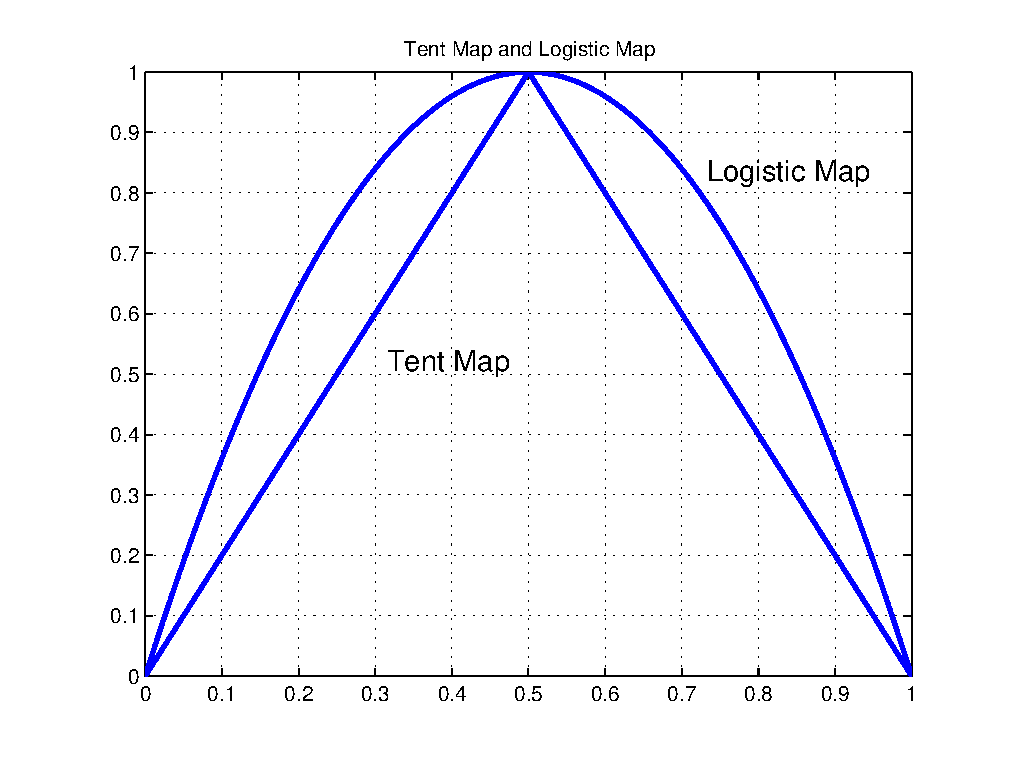
\includegraphics[width=0.35\hsize]{tentmapandlogisticmap.eps}&
  \begin{minipage}[b]{0.6\hsize}
    \textbf{Tent Map}  
     \begin{eqnarray}
        \label{tentmap}
          x' = S_\text{tent}(x) \equiv 1-2|x-\frac{1}{2}|
     \end{eqnarray}
    \textbf{Logistic Map}
     \begin{eqnarray}
        \label{logisticmap}
          x' = S_\text{logistic}(x) \equiv rx(1-x)
     \end{eqnarray}
    Both are known to be chaotic. 
  \end{minipage}
\end{tabular}

\begin{tabular}{cc|l}
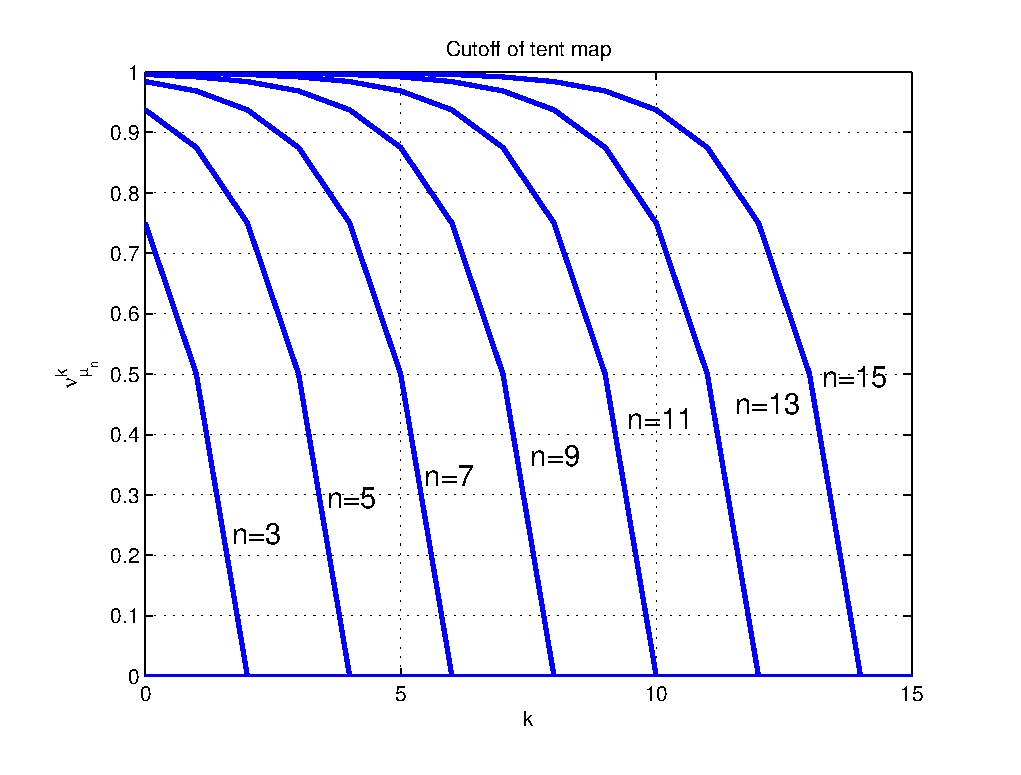
\includegraphics[width=0.3\hsize ,trim=1.2cm 0.8cm 1.2cm 0.8cm,clip]{tentmapcutoff} &
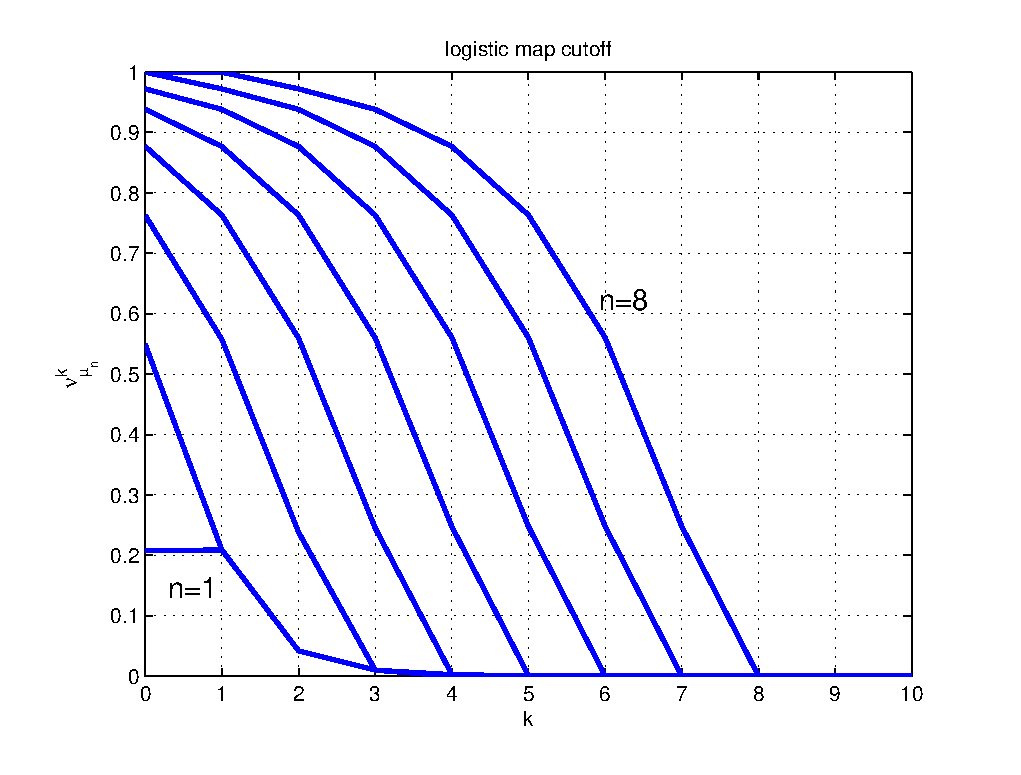
\includegraphics[width=0.3\hsize ,trim=1.2cm 0.8cm 1.2cm 0.8cm,clip]{logisticmapcutoff}&
\begin{minipage}[b]{0.38\hsize}
    \begin{eqnarray}
    \label{tentmapinitial}
    \omega_{\mu_n}^0 = \left\{ \begin{tabular}{c}
                      $\frac{1}{\mu_n}$, \mbox{  if  } $x \le \mu_n$\\ 
                      $0$, \mbox{  otherwise} 
                      \end{tabular}\right.
     \end{eqnarray}
    where $\mu_1 = 1$, and $\mu_{n+1} = \frac{\mu_n}{2}$ for the tent map and $\mu_{n+1}=\frac{1-\sqrt{1-\mu_n}}{2}$ for the logistic map.
\end{minipage} 
\end{tabular}

\vspace{0.5cm}
The above two figures show when the tent map or logistic map is applied to evolve a highly concentrated initial distribution, both of them present sharp changes in total variation distance after a certain number of iterations. The behavior of these chaotic maps are similar to the Markov operators which present cutoffs. However, the shapes of the trajectories are different. 

\vspace{-0.5cm}
\paragraph{Stochastic Symbol Sequence}
Consider $\mathcal{S}=\{0, 1\}$ to be the symbol lists. Let $\Delta$ be the collection of all bi-infinite sequence of elements in $[0,1]$. We define $\delta^0 , \delta^1 \in \Delta$ for each symbol.
\vspace{-1.5cm}

 \begin{eqnarray}
 \delta^0 = \{\cdots \delta_{-n}^0\cdots \delta_{-1}^0.\delta_0^0 \delta_1^0\cdots \delta_n^0\cdots\} \nonumber\\
 \delta^1 = \{\cdots \delta_{-n}^1\cdots \delta_{-1}^1.\delta_0^1 \delta_1^1\cdots \delta_n^1\cdots\}
 \end{eqnarray}
\vspace{-1.6cm}

The interpretation of each $\delta_i^0$ is the probability of $x$ belonging to symbol $0$ after $i$ iterations.
Let $\Omega\in L^\infty[\Lambda], \int_\Lambda \Omega dx=1$ denote the space of probability distribution in $\Lambda$. The map $\psi: \Omega \rightarrow \Delta $ maps a probability distribution $\omega(x) \in \Omega$ to the stochastic symbol sequence $\delta^0$( or $\delta^1$) uniquely. However, it is not invertible. So let us consider a smaller space
\vspace{-1.2cm}

  \begin{eqnarray}
  \bar{\Omega} = \left\{ \omega | \omega(x) = \lim_{n \rightarrow \infty} \prod_{i=-n}^n \delta^{s_i}_i \right\}
  \end{eqnarray}
\vspace{-1.2cm}

where $x$ has symbol sequence $s$. Inside $\bar{\Omega}$, we have $P= \psi^{-1}\circ \sigma \circ \psi$, where $P$ is the Perron-Frobenius operator of the map $S$ with full symbolic dynamics. We can prove the following

\begin{theorem}
$\omega^0 \in \bar{\Omega}$ has stochastic symbol sequence $\delta \equiv \psi(\omega^0)$, such that $\delta_i-\frac{1}{2}$ decreases faster than exponential. Let $p  = \frac{\sum_{i=0}^{\infty} \delta_i}{\delta_{0}}$ and $l = \lfloor p(\delta_{0}-\frac{1}{2})\rfloor$. Then

\vspace{-1.3cm}
  \begin{eqnarray}
    {p \choose l}2^{-p} \ll 1  \Rightarrow |\omega^k-\bar{\omega}|_{TV} \mbox{ presents a sharp change}
  \end{eqnarray}
\end{theorem}

\vspace{-0.8cm}
This result can be extended to $\omega \in \Omega$ such that $|\omega- \psi(\omega)|_{TV}$ is small. 
\vspace{0.3cm}

\begin{tabular}{c|l}
  \begin{tabular}{cc}
  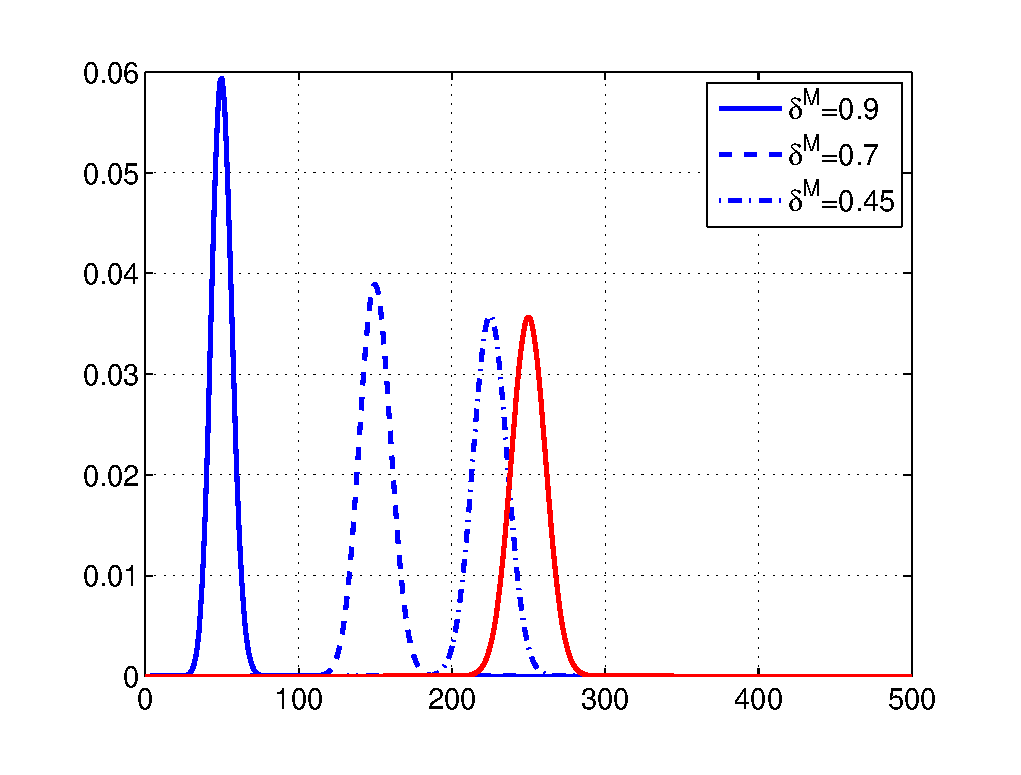
\includegraphics[width=0.26\hsize,trim=0.8cm 0.8cm 0.8cm 0.8cm,clip]{deltaMexample2a} & 
  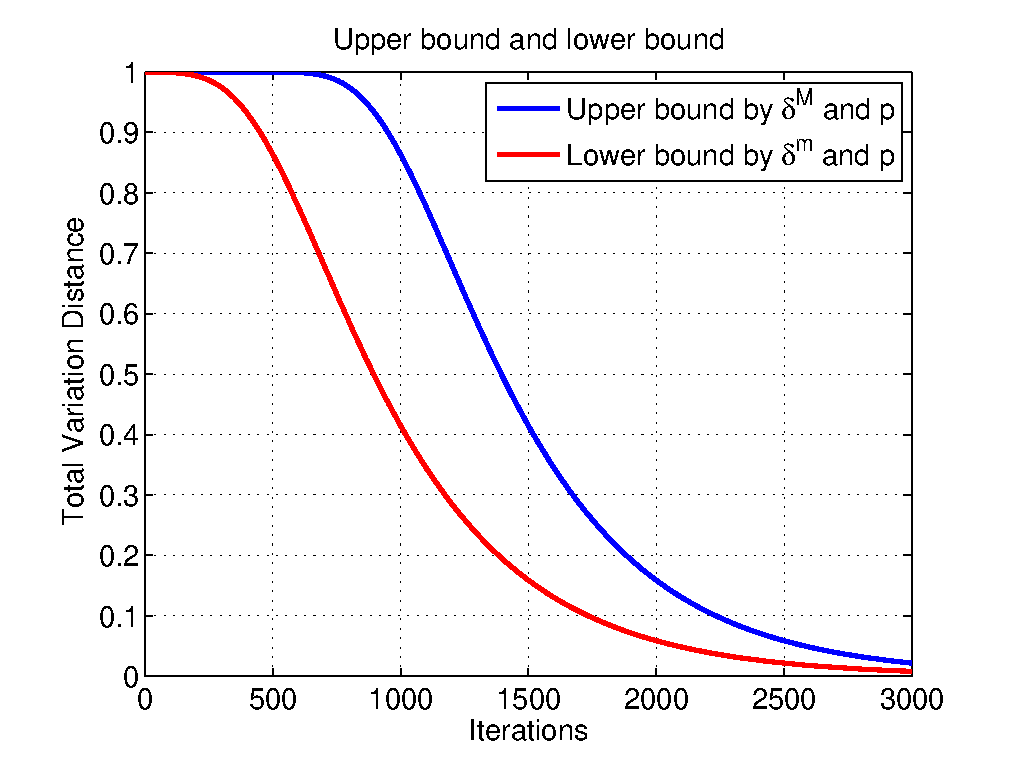
\includegraphics[width=0.26\hsize,trim=0.8cm 0.8cm 0.8cm 0.8cm,clip]{deltaMexample2b} \\
  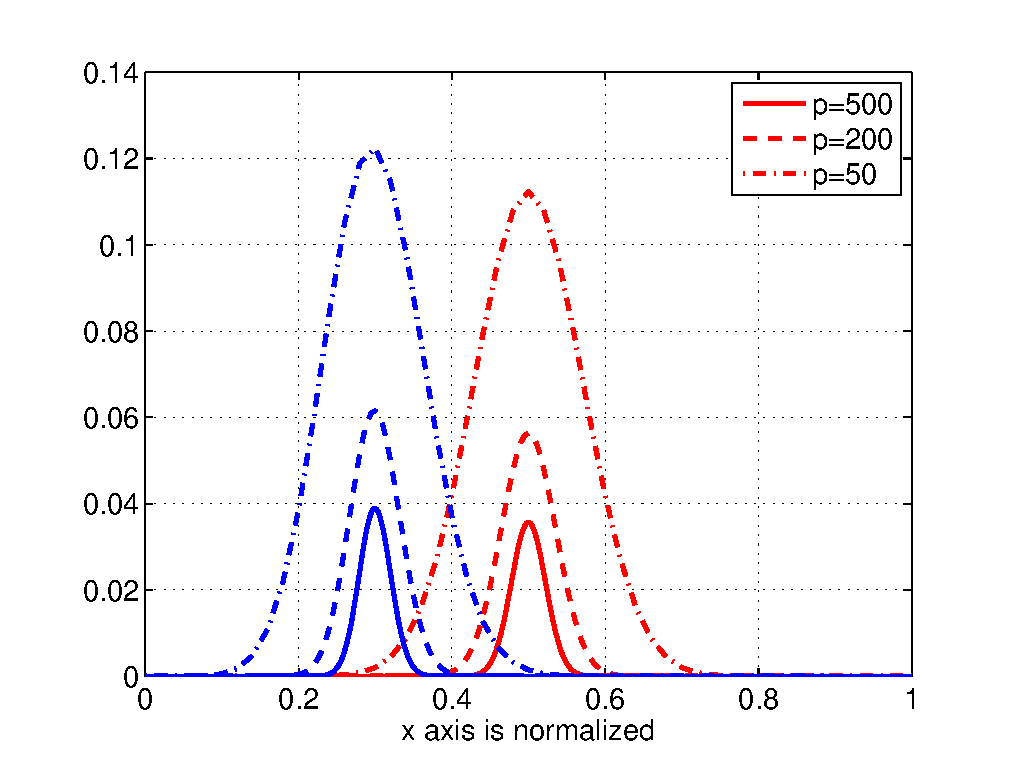
\includegraphics[width=0.26\hsize,trim=0.8cm 0.8cm 0.8cm 0.8cm,clip]{deltaMexample1b} & 
  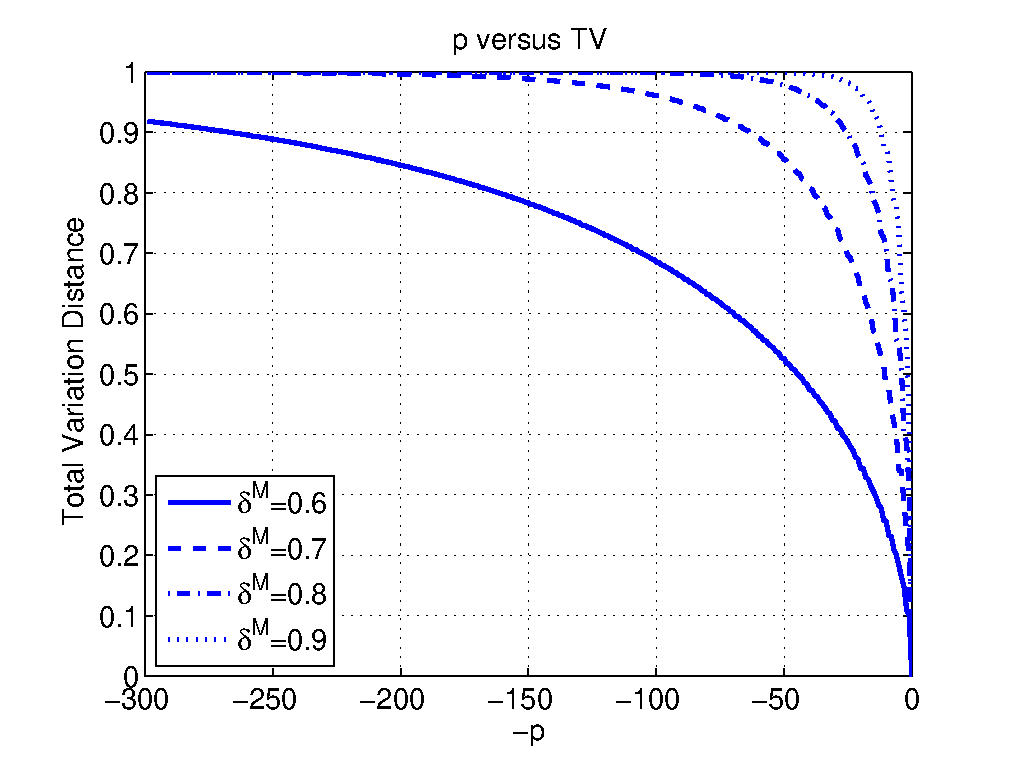
\includegraphics[width=0.26\hsize,trim=0.8cm 0.8cm 0.8cm 0.8cm,clip]{deltaMexample1a} \\
  \end{tabular}&
  \begin{minipage}[s]{0.41\hsize}
   The change of total variation distance can be interpreted as the combination of the two effects: the moving(top two figures) and the reshaping(bottom two figures) of the current distribution to the invariant distribution. The proof of the theorem is done by reducing the system dimension to a smaller space, and then bounding the total variation distances by the difference between two binomial distributions.   
  \end{minipage}
\end{tabular}







%Section ends here
%%%%%%%%%%%%%%%%%%%%%%%%%%%%%%%%%%%%%%%%%%%%%%%%%%%%%%%%%%%%%%%%%%%%%%%%%%%%%%%%%%%%%%%%%%%%%%%%
}
\end{pcolumn}
\begin{pcolumn}{0.32}
%%%%%%%%%%%%%%%%%%%%%%%%%%%%%%%%
%Here is the 3rd column
%%%%%%%%%%%%%%%%%%%%%%%%%%%%%%%%
\pbox{0.9\textwidth}{65cm}{linewidth=4mm,framearc=0.1,linecolor=red,fillstyle=gradient,gradangle=0,gradbegin=white,gradend=white,gradmidpoint=1.0,framesep=1em}{

\begin{center}\pbox{0.8\textwidth}{}{linewidth=2mm,framearc=0.1,linecolor=red,fillstyle=gradient,gradangle=0,gradbegin=white,gradend=whitered,gradmidpoint=1.0,framesep=1em}{\begin{center}\bfseries{\large{Cutoff in Advection-Diffusion Simulation}}\end{center}}\end{center}\vspace{1.25cm}

%%%%%%%%%%%%%%%%%%%%%%%%%%%%%%%%%%%%%%%%%%%%%%%%%%%%%%%%%%%%%%%%%%%%%%%%%%%%%%%%%%%%%%%%%%%%%%%%
%Section begins here

    

\begin{tabular}{c|c}
   \begin{tabular}{l}
   \textbf{Simulation of Standard Map with small diffusion}\\
   \includegraphics[width=0.65\hsize]{demostandardmapcos.eps}
   \end{tabular}&

   \begin{minipage}[s]{0.33\hsize}
    The simulation of $f_n^k = A_n f_n^{k+1}$ with $n = 1000$, $k = 0,2,5,10,20$ and $30$. The colors are mixed quickly in the chaotic region even when the diffusion is small. The bottom figure shows the same simulation without numerical diffusion.    
    
 \centerline{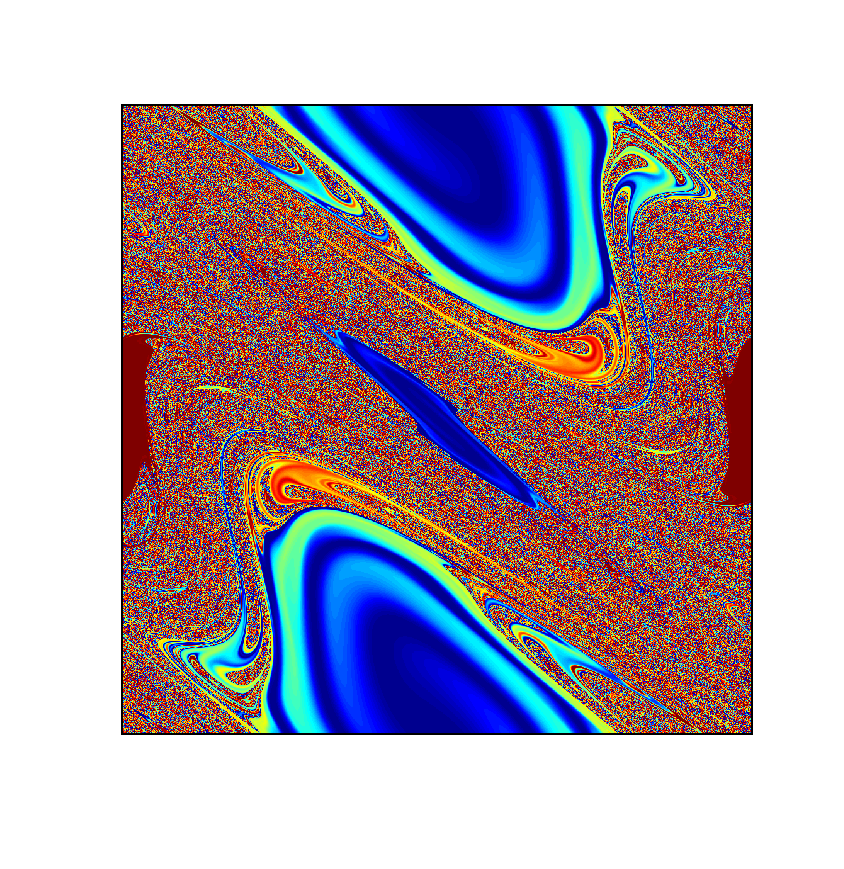
\includegraphics[scale=0.6,angle=90]{standardmapsimuexact2.eps}}
   \end{minipage} 
\end{tabular}



\begin{tabular}{cc|l}
   
        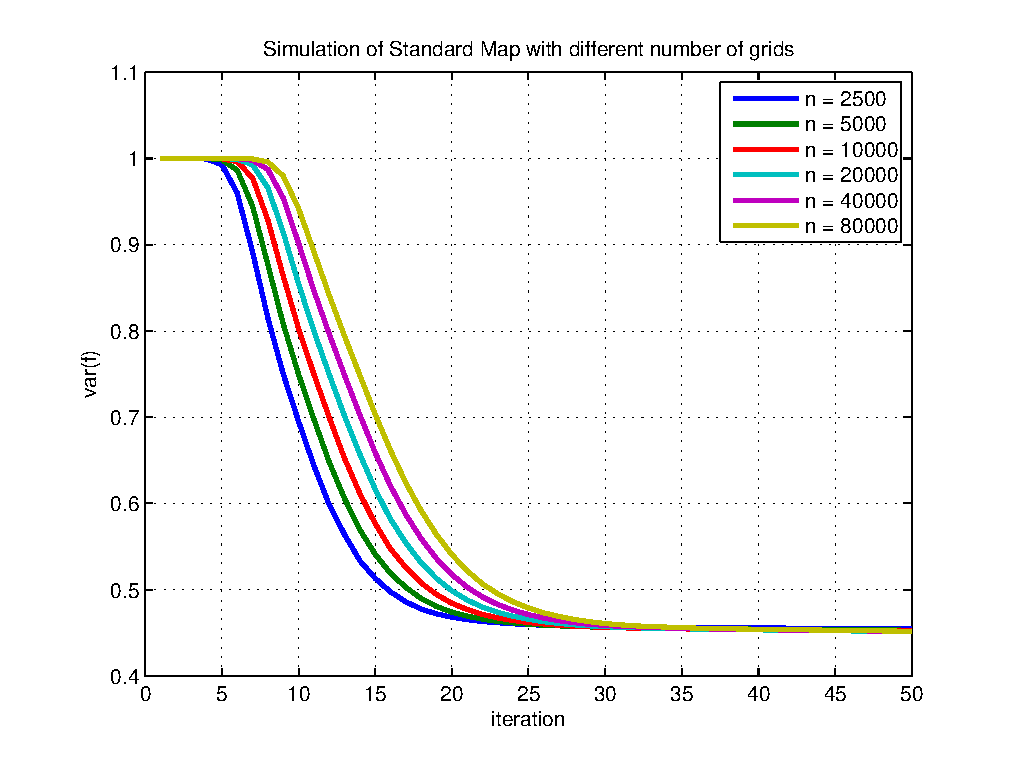
\includegraphics[width=0.35\textwidth,trim=0cm 0cm 0cm 0cm]{standardmapcutoff}&
	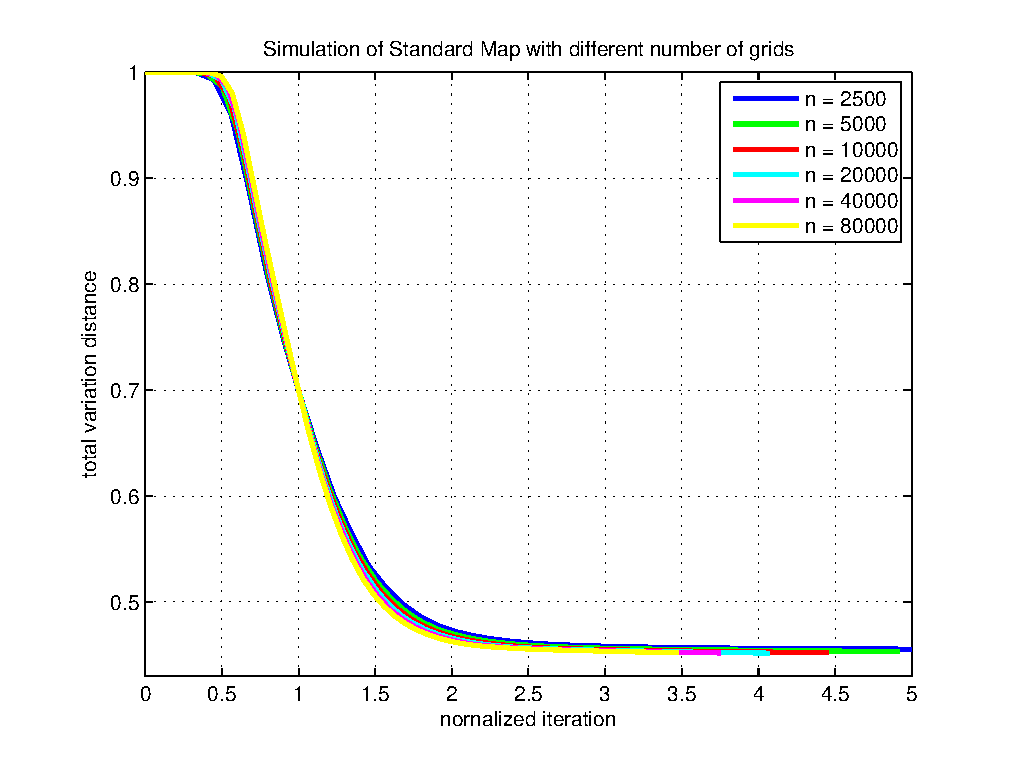
\includegraphics[width=0.35\textwidth,trim=0cm 0cm 0cm 0cm]{standardmapcutoffn}&
   \begin{minipage}[b]{0.28\hsize}
    Now with $n$ varying from $2500$ to $80000$, the total variation versus iteration plot is shown in the left figure. The  trajectories are normalized and plotted again in the right figure. They present a cutoff.
    \end{minipage} 
\end{tabular}


\begin{tabular}{c|l}

  \begin{tabular}{l}
  \textbf{Simulation of a chaotic linked twist map}\\
  \includegraphics[width=0.6\hsize]{example_mixingchannel_app1}
  \end{tabular}&
   \begin{minipage}[s]{0.37\hsize}
    Left figure shows the simulation of the cross sections of a microfluidic mixing channel, which is designed to produce chaotic mixing. The cross sections at $l_x$(channel length)$= 1, 5, 20, 40, 80, 120, 160, 200$ are plotted. The bottom figure shows the total variation distance of the color density also presents a sharp change.   
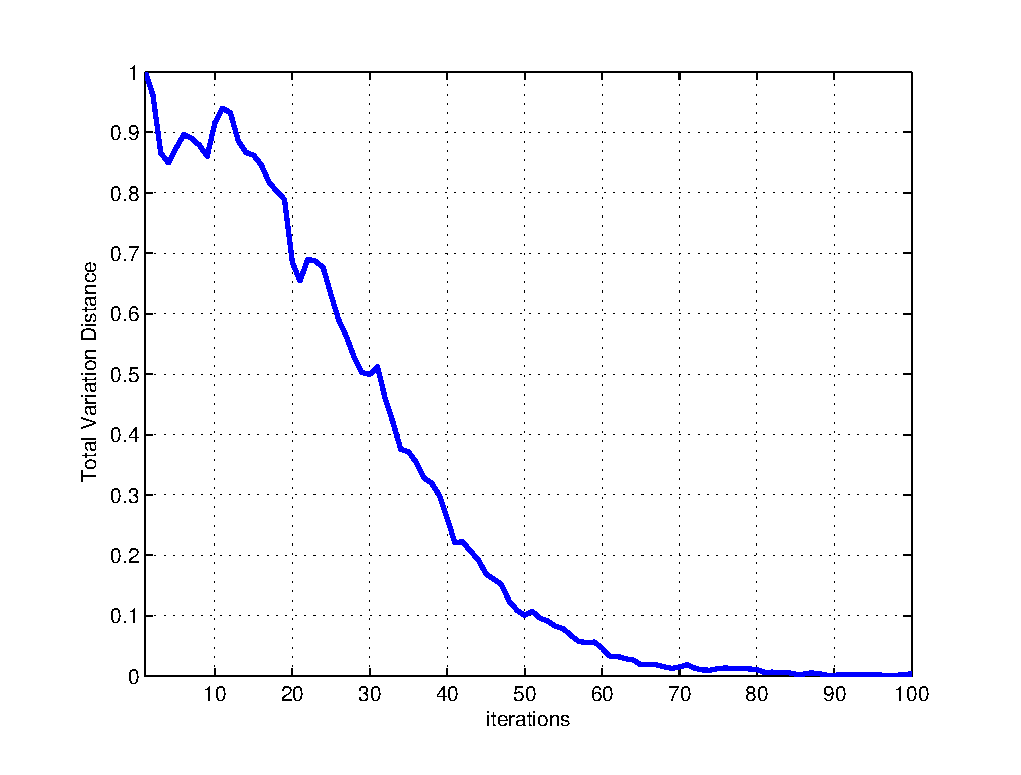
\includegraphics[width=0.9\hsize]{mixingchanneltv} 
    \end{minipage} 


\end{tabular}


%Section ends here
%%%%%%%%%%%%%%%%%%%%%%%%%%%%%%%%%%%%%%%%%%%%%%%%%%%%%%%%%%%%%%%%%%%%%%%%%%%%%%%%%%%%%%%%%%%%%%%%

% Future Work
\begin{center}\pbox{0.8\textwidth}{}{linewidth=2mm,framearc=0.1,linecolor=red,fillstyle=gradient,gradangle=0,gradbegin=white,gradend=whitered,gradmidpoint=1.0,framesep=1em}{\begin{center}\bfseries{\large{Future Work}}\end{center}}\end{center}\vspace{0.5cm}


\begin{itemize}
\item Explore the sharp changes of other measures of certainty/uncertainty besides total variation. 
\item Define a measure of chaos through the happening of the sharp change. 
\end{itemize}

\vspace{-1.5cm}
% References
\bibliographystyle{plain}
\bibliography{mixingbib}
%\nocite{Thiffeault2004}
%\nocite{Mezic2005}



}
\end{pcolumn}
\end{center}



\vspace*{2cm}



\end{poster}

\end{document}

